\documentclass[twoside]{book}

% Packages required by doxygen
\usepackage{fixltx2e}
\usepackage{calc}
\usepackage{doxygen}
\usepackage[export]{adjustbox} % also loads graphicx
\usepackage{graphicx}
\usepackage[utf8]{inputenc}
\usepackage{makeidx}
\usepackage{multicol}
\usepackage{multirow}
\PassOptionsToPackage{warn}{textcomp}
\usepackage{textcomp}
\usepackage[nointegrals]{wasysym}
\usepackage[table]{xcolor}

% Font selection
\usepackage[T1]{fontenc}
\usepackage[scaled=.90]{helvet}
\usepackage{courier}
\usepackage{amssymb}
\usepackage{sectsty}
\renewcommand{\familydefault}{\sfdefault}
\allsectionsfont{%
  \fontseries{bc}\selectfont%
  \color{darkgray}%
}
\renewcommand{\DoxyLabelFont}{%
  \fontseries{bc}\selectfont%
  \color{darkgray}%
}
\newcommand{\+}{\discretionary{\mbox{\scriptsize$\hookleftarrow$}}{}{}}

% Page & text layout
\usepackage{geometry}
\geometry{%
  a4paper,%
  top=2.5cm,%
  bottom=2.5cm,%
  left=2.5cm,%
  right=2.5cm%
}
\tolerance=750
\hfuzz=15pt
\hbadness=750
\setlength{\emergencystretch}{15pt}
\setlength{\parindent}{0cm}
\setlength{\parskip}{3ex plus 2ex minus 2ex}
\makeatletter
\renewcommand{\paragraph}{%
  \@startsection{paragraph}{4}{0ex}{-1.0ex}{1.0ex}{%
    \normalfont\normalsize\bfseries\SS@parafont%
  }%
}
\renewcommand{\subparagraph}{%
  \@startsection{subparagraph}{5}{0ex}{-1.0ex}{1.0ex}{%
    \normalfont\normalsize\bfseries\SS@subparafont%
  }%
}
\makeatother

% Headers & footers
\usepackage{fancyhdr}
\pagestyle{fancyplain}
\fancyhead[LE]{\fancyplain{}{\bfseries\thepage}}
\fancyhead[CE]{\fancyplain{}{}}
\fancyhead[RE]{\fancyplain{}{\bfseries\leftmark}}
\fancyhead[LO]{\fancyplain{}{\bfseries\rightmark}}
\fancyhead[CO]{\fancyplain{}{}}
\fancyhead[RO]{\fancyplain{}{\bfseries\thepage}}
\fancyfoot[LE]{\fancyplain{}{}}
\fancyfoot[CE]{\fancyplain{}{}}
\fancyfoot[RE]{\fancyplain{}{\bfseries\scriptsize Generated by Doxygen }}
\fancyfoot[LO]{\fancyplain{}{\bfseries\scriptsize Generated by Doxygen }}
\fancyfoot[CO]{\fancyplain{}{}}
\fancyfoot[RO]{\fancyplain{}{}}
\renewcommand{\footrulewidth}{0.4pt}
\renewcommand{\chaptermark}[1]{%
  \markboth{#1}{}%
}
\renewcommand{\sectionmark}[1]{%
  \markright{\thesection\ #1}%
}

% Indices & bibliography
\usepackage{natbib}
\usepackage[titles]{tocloft}
\setcounter{tocdepth}{3}
\setcounter{secnumdepth}{5}
\makeindex

% Hyperlinks (required, but should be loaded last)
\usepackage{ifpdf}
\ifpdf
  \usepackage[pdftex,pagebackref=true]{hyperref}
\else
  \usepackage[ps2pdf,pagebackref=true]{hyperref}
\fi
\hypersetup{%
  colorlinks=true,%
  linkcolor=blue,%
  citecolor=blue,%
  unicode%
}

% Custom commands
\newcommand{\clearemptydoublepage}{%
  \newpage{\pagestyle{empty}\cleardoublepage}%
}

\usepackage{caption}
\captionsetup{labelsep=space,justification=centering,font={bf},singlelinecheck=off,skip=4pt,position=top}

%===== C O N T E N T S =====

\begin{document}

% Titlepage & ToC
\hypersetup{pageanchor=false,
             bookmarksnumbered=true,
             pdfencoding=unicode
            }
\pagenumbering{alph}
\begin{titlepage}
\vspace*{7cm}
\begin{center}%
{\Large P\+E\+L\+MA }\\
\vspace*{1cm}
{\large Generated by Doxygen 1.8.13}\\
\end{center}
\end{titlepage}
\clearemptydoublepage
\pagenumbering{roman}
\tableofcontents
\clearemptydoublepage
\pagenumbering{arabic}
\hypersetup{pageanchor=true}

%--- Begin generated contents ---
\chapter{P\+E\+L\+MA}
\label{index}\hypertarget{index}{}\href{https://github.com/ashikaro/Elma}{\tt P\+E\+L\+MA} is a python event loop manager which can be used by embedded and reactive systems application in Python.

The source code for this project is available here \href{https://github.com/ashikaro/Elma}{\tt github}.

\subsection*{Installation }

\begin{DoxyVerb}git clone https://github.com/ashikaro/Elma.git
cd Elma
make build
make run
make docs
\end{DoxyVerb}


\subsection*{Execution }

To run the test process in the container, type \begin{DoxyVerb}python -m unittest
or 
make test
\end{DoxyVerb}


This runs the unit tests we have written for testing a simple process and the test robot.

\subsection*{Testing }

To run tests, do 
\begin{DoxyCode}
make test
\end{DoxyCode}


\subsection*{Architecture }


\begin{DoxyEnumerate}
\item This project is designed to work as an E\+L\+MA python library which can be published to an artifactory and embedded applications can add this as a dependency to incorporate E\+L\+MA into their system.
\end{DoxyEnumerate}
\begin{DoxyEnumerate}
\item All the core E\+L\+MA classes Manger, Process, Event behave functionally the same way as the C++ E\+L\+MA we have built in this class.
\end{DoxyEnumerate}
\begin{DoxyEnumerate}
\item As a proof concept to test if E\+L\+MA can be used in Embedded apps, we have implemented a simple robot which leverage the E\+L\+MA A\+P\+Is to perform simple operations similar to the assignment 7
\end{DoxyEnumerate}

\subsection*{Challenges }


\begin{DoxyEnumerate}
\item Understanding object oriented nuances specific to Python which is a lot different from C++.
\item Steep learning curve considering my inexperience in Python and object oriented languages in general.
\item Implementing virtual methods where we want base class(process) to have no implementation and expect child classes to implement.
\item Python does not have multi argument constructors.
\item Using python closures with nested function for setting up event handling for all the transitions(State\+Machine\textquotesingle{}s init)
\item Writing lambdas in python for event handling.
\end{DoxyEnumerate}

\subsection*{Results }


\begin{DoxyEnumerate}
\item We have written tests for testing Core E\+L\+MA A\+P\+Is and Robot Finite State Machine. Here is the log of the run\+: 
\begin{DoxyCode}
Running tests for core ELMA APIs Using ELMA Manager to test: 1. Initializing a process 2. Scheduling a
       process  3. Updating a process 4. Event handler methods watch and emit
<elma.test.test\_process.TestProcess object at 0x7f329ad3efd0>
watching for hello
watching for pi
emitting hello event

emitting event hello
emitting event hello
emitting pi event

emitting event pi
emitting event pi

Running first set of tests for python client Robot Leveraging ELMA APIs.
Initializing Robot States and making sure states get unique IDs
Id for state Recharge is 0
Id for state Wander is 1
Id for state Find Recharge Station is 2
Id for state Evade is 3
Id for state Make Noise is 4
adding transition for event found recharge station from Find Recharge Station to Recharge
adding transition for event battery full from Recharge to Wander
adding transition for event battery low from Wander to Find Recharge Station
adding transition for event battery low from Evade to Find Recharge Station
adding transition for event start from Wander to Wander
adding transition for event reset from Make Noise to Wander
adding transition for event reset from Evade to Make Noise
adding transition for event intruder detected from Wander to Make Noise
adding transition for event proximity warning from Make Noise to Evade
<elma.api.robot.Robot object at 0x7f329ad3ee48>
watching for found recharge station
watching for battery full
watching for battery low
watching for battery low
watching for start
watching for reset
watching for reset
watching for intruder detected
watching for proximity warning
<elma.api.robot.Robot object at 0x7f329ad3ee48>
calling entry method of Wander
emitting event start
calling exit method of Wander
calling entry method of Wander
Wander
emitting event intruder detected
emitting event intruder detected
calling exit method of Wander
calling entry method of Make Noise
Make Noise
emitting event proximity warning
calling exit method of Make Noise
calling entry method of Evade
Evade
emitting event battery full
Evade
Running First set tests for python client Robot Leveraging ELMA APIs.
Initializing Robot States and making sure states get unique IDs
Id for state Recharge is 5
Id for state Wander is 6
Id for state Find Recharge Station is 7
Id for state Evade is 8
Id for state Make Noise is 9
adding transition for event found recharge station from Find Recharge Station to Recharge
adding transition for event battery full from Recharge to Wander
adding transition for event battery low from Wander to Find Recharge Station
adding transition for event battery low from Evade to Find Recharge Station
adding transition for event start from Wander to Wander
adding transition for event reset from Make Noise to Wander
adding transition for event reset from Evade to Make Noise
adding transition for event intruder detected from Wander to Make Noise
adding transition for event proximity warning from Make Noise to Evade
<elma.api.robot.Robot object at 0x7f329ad02be0>
watching for found recharge station
watching for battery full
watching for battery low
watching for battery low
watching for start
watching for reset
watching for reset
watching for intruder detected
watching for proximity warning
<elma.api.robot.Robot object at 0x7f329ad02be0>
calling entry method of Wander
Wander
emitting event battery low
emitting event battery low
calling exit method of Wander
calling entry method of Find Recharge Station
Find Recharge Station
emitting event found recharge station
calling exit method of Find Recharge Station
calling entry method of Recharge
Recharge
emitting event battery full
calling exit method of Recharge
calling entry method of Wander
Wander
emitting event intruder detected
calling exit method of Wander
calling entry method of Make Noise
Make Noise
emitting event reset
calling exit method of Make Noise
calling entry method of Wander
Wander
emitting event intruder detected
calling exit method of Wander
calling entry method of Make Noise
Make Noise
emitting event proximity warning
calling exit method of Make Noise
calling entry method of Evade
Evade
emitting event battery low
calling exit method of Evade
calling entry method of Find Recharge Station
Find Recharge Station
.
----------------------------------------------------------------------
Ran 3 tests in 0.002s

OK
\end{DoxyCode}

\end{DoxyEnumerate}

\section*{Milestones}

$\ast$\+No changes to the milestones. Going as per the plan.
\begin{DoxyEnumerate}
\item Requirement Analysis, design, scoping by 12th March 2019
\end{DoxyEnumerate}
\begin{DoxyEnumerate}
\item Implement core Elma A\+P\+Is(\+Process,\+Manager) in python by 13th March 2019
\end{DoxyEnumerate}
\begin{DoxyEnumerate}
\item Implement A\+PI\textquotesingle{}s for F\+SM.(State,State Machine) in python by 16th March 2019
\end{DoxyEnumerate}
\begin{DoxyEnumerate}
\item Implement python client using elma to test a simple robot F\+SM by 18th March 2019
\end{DoxyEnumerate}
\begin{DoxyEnumerate}
\item Documentation using Doxygen generated A\+PI descriptions for all classes and methods by 20th March 2019
\end{DoxyEnumerate}

\section*{Current Accomplishments}


\begin{DoxyEnumerate}
\item Accomplished all the milestones.
\end{DoxyEnumerate}

\section*{Resources}


\begin{DoxyItemize}
\item Pluralsight course Python Fundamentals.
\item Py\+Charm I\+DE for Python.
\item Will use C++ elma A\+PI\textquotesingle{}s used in this course as a reference.
\item Unit Tests for hw\+\_\+7, for building test robot finite state machine.
\end{DoxyItemize}

\subsection*{Acknowledgements }

\subsection*{References }


\begin{DoxyEnumerate}
\item Tests not running -\/ \href{https://stackoverflow.com/questions/43957860/python-unittest-ran-0-tests-in-0-000s}{\tt https\+://stackoverflow.\+com/questions/43957860/python-\/unittest-\/ran-\/0-\/tests-\/in-\/0-\/000s} \href{https://stackoverflow.com/questions/7562775/deriving-a-class-from-testcase-throws-two-errors}{\tt https\+://stackoverflow.\+com/questions/7562775/deriving-\/a-\/class-\/from-\/testcase-\/throws-\/two-\/errors}
\item Docker not able to bring bash shell up. Instead used sh \href{https://stackoverflow.com/questions/27959011/why-does-docker-say-it-cant-execute-bash}{\tt https\+://stackoverflow.\+com/questions/27959011/why-\/does-\/docker-\/say-\/it-\/cant-\/execute-\/bash}
\item Docker image for Python reference \href{https://blog.realkinetic.com/building-minimal-docker-containers-for-python-applications-37d0272c52f3}{\tt https\+://blog.\+realkinetic.\+com/building-\/minimal-\/docker-\/containers-\/for-\/python-\/applications-\/37d0272c52f3}
\item Python time in milliseconds \href{https://blog.realkinetic.com/building-minimal-docker-containers-for-python-applications-37d0272c52f3}{\tt https\+://blog.\+realkinetic.\+com/building-\/minimal-\/docker-\/containers-\/for-\/python-\/applications-\/37d0272c52f3}
\item Declaring static variables \href{https://www.geeksforgeeks.org/g-fact-34-class-or-static-variables-in-python/}{\tt https\+://www.\+geeksforgeeks.\+org/g-\/fact-\/34-\/class-\/or-\/static-\/variables-\/in-\/python/}
\item Inner functions and closures for event handling \href{https://realpython.com/inner-functions-what-are-they-good-for/}{\tt https\+://realpython.\+com/inner-\/functions-\/what-\/are-\/they-\/good-\/for/} 
\end{DoxyEnumerate}
\chapter{Namespace Index}
\section{Namespace List}
Here is a list of all documented namespaces with brief descriptions\+:\begin{DoxyCompactList}
\item\contentsline{section}{\hyperlink{namespaceelma_1_1api_1_1event}{elma.\+api.\+event} \\*This module has the class definition for the \hyperlink{classelma_1_1api_1_1event_1_1Event}{Event} class }{\pageref{namespaceelma_1_1api_1_1event}}{}
\item\contentsline{section}{\hyperlink{namespaceelma_1_1test_1_1test__process}{elma.\+test.\+test\+\_\+process} \\*This module contains the class definition for \hyperlink{classelma_1_1test_1_1test__process_1_1TestProcess}{Test\+Process} }{\pageref{namespaceelma_1_1test_1_1test__process}}{}
\end{DoxyCompactList}

\chapter{Hierarchical Index}
\section{Class Hierarchy}
This inheritance list is sorted roughly, but not completely, alphabetically\+:\begin{DoxyCompactList}
\item \contentsline{section}{elma.\+api.\+event.\+Event}{\pageref{classelma_1_1api_1_1event_1_1Event}}{}
\item \contentsline{section}{elma.\+api.\+manager.\+Manager}{\pageref{classelma_1_1api_1_1manager_1_1Manager}}{}
\item \contentsline{section}{elma.\+api.\+process.\+Process}{\pageref{classelma_1_1api_1_1process_1_1Process}}{}
\begin{DoxyCompactList}
\item \contentsline{section}{elma.\+api.\+state\+\_\+machine.\+State\+Machine}{\pageref{classelma_1_1api_1_1state__machine_1_1StateMachine}}{}
\begin{DoxyCompactList}
\item \contentsline{section}{elma.\+api.\+robot.\+Robot}{\pageref{classelma_1_1api_1_1robot_1_1Robot}}{}
\end{DoxyCompactList}
\item \contentsline{section}{elma.\+test.\+test\+\_\+process.\+Test\+Process}{\pageref{classelma_1_1test_1_1test__process_1_1TestProcess}}{}
\end{DoxyCompactList}
\item \contentsline{section}{elma.\+api.\+state.\+State}{\pageref{classelma_1_1api_1_1state_1_1State}}{}
\begin{DoxyCompactList}
\item \contentsline{section}{elma.\+api.\+robot.\+Robot\+State}{\pageref{classelma_1_1api_1_1robot_1_1RobotState}}{}
\end{DoxyCompactList}
\item Test\+Case\begin{DoxyCompactList}
\item \contentsline{section}{elma.\+test.\+test\+\_\+elma.\+Test\+Elma}{\pageref{classelma_1_1test_1_1test__elma_1_1TestElma}}{}
\end{DoxyCompactList}
\item \contentsline{section}{elma.\+api.\+transition.\+Transition}{\pageref{classelma_1_1api_1_1transition_1_1Transition}}{}
\item Enum\begin{DoxyCompactList}
\item \contentsline{section}{elma.\+api.\+process.\+Status\+\_\+\+Type}{\pageref{classelma_1_1api_1_1process_1_1Status__Type}}{}
\end{DoxyCompactList}
\end{DoxyCompactList}

\chapter{Class Index}
\section{Class List}
Here are the classes, structs, unions and interfaces with brief descriptions\+:\begin{DoxyCompactList}
\item\contentsline{section}{\hyperlink{classelma_1_1api_1_1event_1_1Event}{elma.\+api.\+event.\+Event} \\*Events that can be emitted, watched, and responded to with event handlers }{\pageref{classelma_1_1api_1_1event_1_1Event}}{}
\item\contentsline{section}{\hyperlink{classelma_1_1api_1_1manager_1_1Manager}{elma.\+api.\+manager.\+Manager} }{\pageref{classelma_1_1api_1_1manager_1_1Manager}}{}
\item\contentsline{section}{\hyperlink{classelma_1_1api_1_1process_1_1Process}{elma.\+api.\+process.\+Process} }{\pageref{classelma_1_1api_1_1process_1_1Process}}{}
\item\contentsline{section}{\hyperlink{classelma_1_1api_1_1robot_1_1Robot}{elma.\+api.\+robot.\+Robot} }{\pageref{classelma_1_1api_1_1robot_1_1Robot}}{}
\item\contentsline{section}{\hyperlink{classelma_1_1api_1_1robot_1_1RobotState}{elma.\+api.\+robot.\+Robot\+State} }{\pageref{classelma_1_1api_1_1robot_1_1RobotState}}{}
\item\contentsline{section}{\hyperlink{classelma_1_1api_1_1state_1_1State}{elma.\+api.\+state.\+State} }{\pageref{classelma_1_1api_1_1state_1_1State}}{}
\item\contentsline{section}{\hyperlink{classelma_1_1api_1_1state__machine_1_1StateMachine}{elma.\+api.\+state\+\_\+machine.\+State\+Machine} }{\pageref{classelma_1_1api_1_1state__machine_1_1StateMachine}}{}
\item\contentsline{section}{\hyperlink{classelma_1_1api_1_1process_1_1Status__Type}{elma.\+api.\+process.\+Status\+\_\+\+Type} }{\pageref{classelma_1_1api_1_1process_1_1Status__Type}}{}
\item\contentsline{section}{\hyperlink{classelma_1_1test_1_1test__elma_1_1TestElma}{elma.\+test.\+test\+\_\+elma.\+Test\+Elma} }{\pageref{classelma_1_1test_1_1test__elma_1_1TestElma}}{}
\item\contentsline{section}{\hyperlink{classelma_1_1test_1_1test__process_1_1TestProcess}{elma.\+test.\+test\+\_\+process.\+Test\+Process} \\*This is a test process class inheriting the Process class to test the working of the E\+L\+MA process A\+P\+Is }{\pageref{classelma_1_1test_1_1test__process_1_1TestProcess}}{}
\item\contentsline{section}{\hyperlink{classelma_1_1api_1_1transition_1_1Transition}{elma.\+api.\+transition.\+Transition} }{\pageref{classelma_1_1api_1_1transition_1_1Transition}}{}
\end{DoxyCompactList}

\chapter{Namespace Documentation}
\hypertarget{namespaceelma_1_1api_1_1event}{}\section{elma.\+api.\+event Namespace Reference}
\label{namespaceelma_1_1api_1_1event}\index{elma.\+api.\+event@{elma.\+api.\+event}}


This module has the class definition for the \hyperlink{classelma_1_1api_1_1event_1_1Event}{Event} class.  


\subsection*{Classes}
\begin{DoxyCompactItemize}
\item 
class \hyperlink{classelma_1_1api_1_1event_1_1Event}{Event}
\begin{DoxyCompactList}\small\item\em Events that can be emitted, watched, and responded to with event handlers. \end{DoxyCompactList}\end{DoxyCompactItemize}


\subsection{Detailed Description}
This module has the class definition for the \hyperlink{classelma_1_1api_1_1event_1_1Event}{Event} class. 

More details. 
\hypertarget{namespaceelma_1_1test_1_1test__process}{}\section{elma.\+test.\+test\+\_\+process Namespace Reference}
\label{namespaceelma_1_1test_1_1test__process}\index{elma.\+test.\+test\+\_\+process@{elma.\+test.\+test\+\_\+process}}


This module contains the class definition for \hyperlink{classelma_1_1test_1_1test__process_1_1TestProcess}{Test\+Process}.  


\subsection*{Classes}
\begin{DoxyCompactItemize}
\item 
class \hyperlink{classelma_1_1test_1_1test__process_1_1TestProcess}{Test\+Process}
\begin{DoxyCompactList}\small\item\em This is a test process class inheriting the Process class to test the working of the E\+L\+MA process A\+P\+Is. \end{DoxyCompactList}\end{DoxyCompactItemize}


\subsection{Detailed Description}
This module contains the class definition for \hyperlink{classelma_1_1test_1_1test__process_1_1TestProcess}{Test\+Process}. 


\chapter{Class Documentation}
\hypertarget{classelma_1_1api_1_1event_1_1Event}{}\section{elma.\+api.\+event.\+Event Class Reference}
\label{classelma_1_1api_1_1event_1_1Event}\index{elma.\+api.\+event.\+Event@{elma.\+api.\+event.\+Event}}


Events that can be emitted, watched, and responded to with event handlers.  


\subsection*{Public Member Functions}
\begin{DoxyCompactItemize}
\item 
\mbox{\Hypertarget{classelma_1_1api_1_1event_1_1Event_aed8d4b5c4d860cfd15b66cf7137395a3}\label{classelma_1_1api_1_1event_1_1Event_aed8d4b5c4d860cfd15b66cf7137395a3}} 
def {\bfseries \+\_\+\+\_\+init\+\_\+\+\_\+} (self, \hyperlink{classelma_1_1api_1_1event_1_1Event_aff9b51b4633b58b32e4cb04d9fca568d}{name}=None, \hyperlink{classelma_1_1api_1_1event_1_1Event_a26e3c222b0421cd70d66041466e0b189}{value}=0)
\item 
def \hyperlink{classelma_1_1api_1_1event_1_1Event_aff9b51b4633b58b32e4cb04d9fca568d}{name} (self)
\begin{DoxyCompactList}\small\item\em return the name of the event \end{DoxyCompactList}\item 
def \hyperlink{classelma_1_1api_1_1event_1_1Event_a5912a8957bf49373f95a5646c861a905}{propagate} (self)
\begin{DoxyCompactList}\small\item\em Determine whether the event will propagate to the next event handlert. \end{DoxyCompactList}\item 
def \hyperlink{classelma_1_1api_1_1event_1_1Event_a2b670f52655e83d9ab9f80385f5917ff}{stop\+\_\+propagation} (self)
\begin{DoxyCompactList}\small\item\em Prevent the event from propagating to the next event handler. \end{DoxyCompactList}\item 
\mbox{\Hypertarget{classelma_1_1api_1_1event_1_1Event_a5b44cfed288e84f52d13b9082fe09b5c}\label{classelma_1_1api_1_1event_1_1Event_a5b44cfed288e84f52d13b9082fe09b5c}} 
def {\bfseries reset} (self)
\item 
\mbox{\Hypertarget{classelma_1_1api_1_1event_1_1Event_a31067ddfc1b3a5584799255db0405efb}\label{classelma_1_1api_1_1event_1_1Event_a31067ddfc1b3a5584799255db0405efb}} 
def \hyperlink{classelma_1_1api_1_1event_1_1Event_a31067ddfc1b3a5584799255db0405efb}{empty} (self)
\begin{DoxyCompactList}\small\item\em Determine whether the event has no data return Whether the event has no data. \end{DoxyCompactList}\item 
\mbox{\Hypertarget{classelma_1_1api_1_1event_1_1Event_a26e3c222b0421cd70d66041466e0b189}\label{classelma_1_1api_1_1event_1_1Event_a26e3c222b0421cd70d66041466e0b189}} 
def \hyperlink{classelma_1_1api_1_1event_1_1Event_a26e3c222b0421cd70d66041466e0b189}{value} (self)
\begin{DoxyCompactList}\small\item\em Get the data value associated with an event return The value. \end{DoxyCompactList}\end{DoxyCompactItemize}


\subsection{Detailed Description}
Events that can be emitted, watched, and responded to with event handlers. 

Events are constructed with a jsonable value, as in 
\begin{DoxyCode}
Event(3.14);
Event(\textcolor{stringliteral}{"hello world"});
Event(\{1,2,3\});
\end{DoxyCode}
 

\subsection{Member Function Documentation}
\mbox{\Hypertarget{classelma_1_1api_1_1event_1_1Event_aff9b51b4633b58b32e4cb04d9fca568d}\label{classelma_1_1api_1_1event_1_1Event_aff9b51b4633b58b32e4cb04d9fca568d}} 
\index{elma\+::api\+::event\+::\+Event@{elma\+::api\+::event\+::\+Event}!name@{name}}
\index{name@{name}!elma\+::api\+::event\+::\+Event@{elma\+::api\+::event\+::\+Event}}
\subsubsection{\texorpdfstring{name()}{name()}}
{\footnotesize\ttfamily def elma.\+api.\+event.\+Event.\+name (\begin{DoxyParamCaption}\item[{}]{self }\end{DoxyParamCaption})}



return the name of the event 


\begin{DoxyParams}{Parameters}
{\em self} & The object pointer. \\
\hline
\end{DoxyParams}
\mbox{\Hypertarget{classelma_1_1api_1_1event_1_1Event_a5912a8957bf49373f95a5646c861a905}\label{classelma_1_1api_1_1event_1_1Event_a5912a8957bf49373f95a5646c861a905}} 
\index{elma\+::api\+::event\+::\+Event@{elma\+::api\+::event\+::\+Event}!propagate@{propagate}}
\index{propagate@{propagate}!elma\+::api\+::event\+::\+Event@{elma\+::api\+::event\+::\+Event}}
\subsubsection{\texorpdfstring{propagate()}{propagate()}}
{\footnotesize\ttfamily def elma.\+api.\+event.\+Event.\+propagate (\begin{DoxyParamCaption}\item[{}]{self }\end{DoxyParamCaption})}



Determine whether the event will propagate to the next event handlert. 


\begin{DoxyParams}{Parameters}
{\em self} & The object pointer. \\
\hline
\end{DoxyParams}
\mbox{\Hypertarget{classelma_1_1api_1_1event_1_1Event_a2b670f52655e83d9ab9f80385f5917ff}\label{classelma_1_1api_1_1event_1_1Event_a2b670f52655e83d9ab9f80385f5917ff}} 
\index{elma\+::api\+::event\+::\+Event@{elma\+::api\+::event\+::\+Event}!stop\+\_\+propagation@{stop\+\_\+propagation}}
\index{stop\+\_\+propagation@{stop\+\_\+propagation}!elma\+::api\+::event\+::\+Event@{elma\+::api\+::event\+::\+Event}}
\subsubsection{\texorpdfstring{stop\+\_\+propagation()}{stop\_propagation()}}
{\footnotesize\ttfamily def elma.\+api.\+event.\+Event.\+stop\+\_\+propagation (\begin{DoxyParamCaption}\item[{}]{self }\end{DoxyParamCaption})}



Prevent the event from propagating to the next event handler. 

Typically called within an event handler to prevent an subsequent events that are watching the same event from firing. 

The documentation for this class was generated from the following file\+:\begin{DoxyCompactItemize}
\item 
elma/api/event.\+py\end{DoxyCompactItemize}

\hypertarget{classelma_1_1api_1_1manager_1_1Manager}{}\section{elma.\+api.\+manager.\+Manager Class Reference}
\label{classelma_1_1api_1_1manager_1_1Manager}\index{elma.\+api.\+manager.\+Manager@{elma.\+api.\+manager.\+Manager}}
\subsection*{Public Member Functions}
\begin{DoxyCompactItemize}
\item 
\mbox{\Hypertarget{classelma_1_1api_1_1manager_1_1Manager_af6ea4ce84e82ccc172774bb1ded3d3b0}\label{classelma_1_1api_1_1manager_1_1Manager_af6ea4ce84e82ccc172774bb1ded3d3b0}} 
def {\bfseries \+\_\+\+\_\+init\+\_\+\+\_\+} (self)
\item 
\mbox{\Hypertarget{classelma_1_1api_1_1manager_1_1Manager_afa7d8aad0d3fb8bc2da697ee251d8f66}\label{classelma_1_1api_1_1manager_1_1Manager_afa7d8aad0d3fb8bc2da697ee251d8f66}} 
def {\bfseries schedule} (self, process, period)
\item 
\mbox{\Hypertarget{classelma_1_1api_1_1manager_1_1Manager_adfd5bd95cca1ebfba742319c1d01e4e2}\label{classelma_1_1api_1_1manager_1_1Manager_adfd5bd95cca1ebfba742319c1d01e4e2}} 
def {\bfseries start\+\_\+time} (self)
\item 
\mbox{\Hypertarget{classelma_1_1api_1_1manager_1_1Manager_ad26dad0553c0e6936acbedba79b38bda}\label{classelma_1_1api_1_1manager_1_1Manager_ad26dad0553c0e6936acbedba79b38bda}} 
def {\bfseries elapsed} (self)
\item 
\mbox{\Hypertarget{classelma_1_1api_1_1manager_1_1Manager_a79300fdc4b141009a2c34648b566f216}\label{classelma_1_1api_1_1manager_1_1Manager_a79300fdc4b141009a2c34648b566f216}} 
def {\bfseries watch} (self, event\+\_\+name, handler)
\item 
\mbox{\Hypertarget{classelma_1_1api_1_1manager_1_1Manager_a8c842ef67392a11900ce089e05b23c58}\label{classelma_1_1api_1_1manager_1_1Manager_a8c842ef67392a11900ce089e05b23c58}} 
def {\bfseries emit} (self, event)
\item 
\mbox{\Hypertarget{classelma_1_1api_1_1manager_1_1Manager_a4e451c5cd548a0086536fa9c990b338e}\label{classelma_1_1api_1_1manager_1_1Manager_a4e451c5cd548a0086536fa9c990b338e}} 
def {\bfseries all} (self, f)
\item 
\mbox{\Hypertarget{classelma_1_1api_1_1manager_1_1Manager_a724e1c80f53aff3430bc465a5671ddee}\label{classelma_1_1api_1_1manager_1_1Manager_a724e1c80f53aff3430bc465a5671ddee}} 
def {\bfseries init} (self)
\item 
\mbox{\Hypertarget{classelma_1_1api_1_1manager_1_1Manager_a7e9916576b109e0d633c55e3854d1b78}\label{classelma_1_1api_1_1manager_1_1Manager_a7e9916576b109e0d633c55e3854d1b78}} 
def {\bfseries start} (self)
\item 
\mbox{\Hypertarget{classelma_1_1api_1_1manager_1_1Manager_a0feb4a517ab5840dcb6d8e15d33f22be}\label{classelma_1_1api_1_1manager_1_1Manager_a0feb4a517ab5840dcb6d8e15d33f22be}} 
def {\bfseries stop} (self)
\item 
\mbox{\Hypertarget{classelma_1_1api_1_1manager_1_1Manager_acb942259598dffdb074bea5171f0e2e9}\label{classelma_1_1api_1_1manager_1_1Manager_acb942259598dffdb074bea5171f0e2e9}} 
def {\bfseries update} (self)
\item 
\mbox{\Hypertarget{classelma_1_1api_1_1manager_1_1Manager_a241f798dcfb0cda2a47d744d8713c456}\label{classelma_1_1api_1_1manager_1_1Manager_a241f798dcfb0cda2a47d744d8713c456}} 
def {\bfseries run} (self, runtime)
\item 
\mbox{\Hypertarget{classelma_1_1api_1_1manager_1_1Manager_ab077b5cf1492213bc057f6a19fc78950}\label{classelma_1_1api_1_1manager_1_1Manager_ab077b5cf1492213bc057f6a19fc78950}} 
def {\bfseries get\+\_\+milliseconds} (self, duration)
\end{DoxyCompactItemize}
\subsection*{Public Attributes}
\begin{DoxyCompactItemize}
\item 
\mbox{\Hypertarget{classelma_1_1api_1_1manager_1_1Manager_a7ec673d8f79675c813f7a5aca8adab8d}\label{classelma_1_1api_1_1manager_1_1Manager_a7ec673d8f79675c813f7a5aca8adab8d}} 
{\bfseries event\+\_\+handlers}
\end{DoxyCompactItemize}


The documentation for this class was generated from the following file\+:\begin{DoxyCompactItemize}
\item 
elma/api/manager.\+py\end{DoxyCompactItemize}

\hypertarget{classelma_1_1api_1_1process_1_1Process}{}\section{elma.\+api.\+process.\+Process Class Reference}
\label{classelma_1_1api_1_1process_1_1Process}\index{elma.\+api.\+process.\+Process@{elma.\+api.\+process.\+Process}}


abstract base class  


Inheritance diagram for elma.\+api.\+process.\+Process\+:\begin{figure}[H]
\begin{center}
\leavevmode
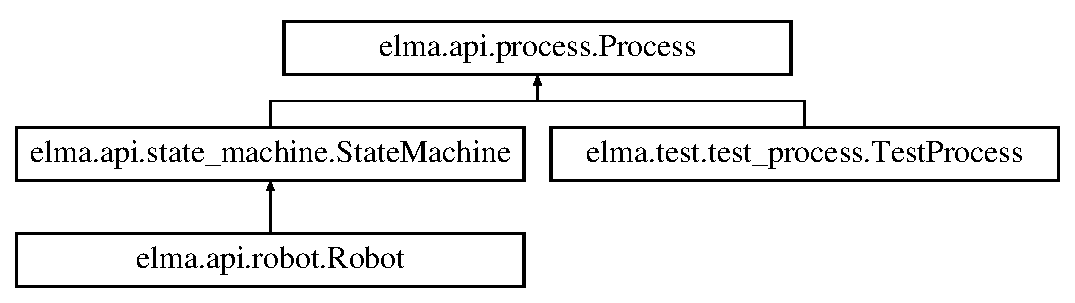
\includegraphics[height=3.000000cm]{classelma_1_1api_1_1process_1_1Process}
\end{center}
\end{figure}
\subsection*{Public Member Functions}
\begin{DoxyCompactItemize}
\item 
def \hyperlink{classelma_1_1api_1_1process_1_1Process_a7a539964a64e16cc8bc42e15124df35e}{\+\_\+\+\_\+init\+\_\+\+\_\+} (self, \hyperlink{classelma_1_1api_1_1process_1_1Process_affa061fab12e699d4d04471bfaf52a1a}{name}=None, \hyperlink{classelma_1_1api_1_1process_1_1Process_a6dc2725cd3d032b3ec80e0fc6c52a994}{status}=None, manager=None)
\begin{DoxyCompactList}\small\item\em Status of the process, as managed by a Manager. \end{DoxyCompactList}\item 
\mbox{\Hypertarget{classelma_1_1api_1_1process_1_1Process_a04c3be5718b17eac25b42779ea368793}\label{classelma_1_1api_1_1process_1_1Process_a04c3be5718b17eac25b42779ea368793}} 
def {\bfseries init} (self)
\item 
\mbox{\Hypertarget{classelma_1_1api_1_1process_1_1Process_a61245c078eec81fa9ce79105942e7cb3}\label{classelma_1_1api_1_1process_1_1Process_a61245c078eec81fa9ce79105942e7cb3}} 
def {\bfseries start} (self)
\item 
\mbox{\Hypertarget{classelma_1_1api_1_1process_1_1Process_ab95818df6159186c9d286963ad561da1}\label{classelma_1_1api_1_1process_1_1Process_ab95818df6159186c9d286963ad561da1}} 
def {\bfseries update} (self)
\item 
\mbox{\Hypertarget{classelma_1_1api_1_1process_1_1Process_a2751375eb541bb0dae8211d4b692b4fc}\label{classelma_1_1api_1_1process_1_1Process_a2751375eb541bb0dae8211d4b692b4fc}} 
def {\bfseries stop} (self)
\item 
def \hyperlink{classelma_1_1api_1_1process_1_1Process_a8e37ba949b3285fe52ca8638cdcb0bb9}{period} (self)
\begin{DoxyCompactList}\small\item\em Getter. \end{DoxyCompactList}\item 
def \hyperlink{classelma_1_1api_1_1process_1_1Process_a6dc2725cd3d032b3ec80e0fc6c52a994}{status} (self)
\begin{DoxyCompactList}\small\item\em Getter. \end{DoxyCompactList}\item 
def \hyperlink{classelma_1_1api_1_1process_1_1Process_affa061fab12e699d4d04471bfaf52a1a}{name} (self)
\begin{DoxyCompactList}\small\item\em Getter. \end{DoxyCompactList}\item 
def \hyperlink{classelma_1_1api_1_1process_1_1Process_ad0a58ddb9103ec226c42892e5a3d2c3f}{num\+\_\+updates} (self)
\begin{DoxyCompactList}\small\item\em Getter. \end{DoxyCompactList}\item 
def \hyperlink{classelma_1_1api_1_1process_1_1Process_aa37c2ece596b3580990332709564345f}{start\+\_\+time} (self)
\begin{DoxyCompactList}\small\item\em Getter. \end{DoxyCompactList}\item 
def \hyperlink{classelma_1_1api_1_1process_1_1Process_aef00f41f3c8bab2b49329d05ce83f534}{last\+\_\+update} (self)
\begin{DoxyCompactList}\small\item\em Getter. \end{DoxyCompactList}\item 
def \hyperlink{classelma_1_1api_1_1process_1_1Process_a47488e16165e28243766c7a6f5a51e32}{previous\+\_\+update} (self)
\begin{DoxyCompactList}\small\item\em Getter. \end{DoxyCompactList}\item 
def \hyperlink{classelma_1_1api_1_1process_1_1Process_a65c2b15f6f42435a532aafd62631cc1d}{milli\+\_\+time} (self)
\begin{DoxyCompactList}\small\item\em The time since the last update in millisconds, as a double. \end{DoxyCompactList}\item 
\mbox{\Hypertarget{classelma_1_1api_1_1process_1_1Process_abbe3f746bdaa56b1166e37c6622e93f9}\label{classelma_1_1api_1_1process_1_1Process_abbe3f746bdaa56b1166e37c6622e93f9}} 
def {\bfseries diff\+\_\+count} (self)
\item 
\mbox{\Hypertarget{classelma_1_1api_1_1process_1_1Process_afb8d0a01fbbf47d20fdd97d3b9d0e2e9}\label{classelma_1_1api_1_1process_1_1Process_afb8d0a01fbbf47d20fdd97d3b9d0e2e9}} 
def {\bfseries watch} (self, event\+\_\+name, handler)
\item 
\mbox{\Hypertarget{classelma_1_1api_1_1process_1_1Process_aaefd6d23649bf1bb0674dad7e2cebef8}\label{classelma_1_1api_1_1process_1_1Process_aaefd6d23649bf1bb0674dad7e2cebef8}} 
def {\bfseries emit} (self, event)
\end{DoxyCompactItemize}
\subsection*{Public Attributes}
\begin{DoxyCompactItemize}
\item 
\mbox{\Hypertarget{classelma_1_1api_1_1process_1_1Process_a37f72d81499fbbf8a3beaeff06d62202}\label{classelma_1_1api_1_1process_1_1Process_a37f72d81499fbbf8a3beaeff06d62202}} 
{\bfseries diff\+\_\+count}
\end{DoxyCompactItemize}


\subsection{Detailed Description}
abstract base class 

\subsection{Constructor \& Destructor Documentation}
\mbox{\Hypertarget{classelma_1_1api_1_1process_1_1Process_a7a539964a64e16cc8bc42e15124df35e}\label{classelma_1_1api_1_1process_1_1Process_a7a539964a64e16cc8bc42e15124df35e}} 
\index{elma\+::api\+::process\+::\+Process@{elma\+::api\+::process\+::\+Process}!\+\_\+\+\_\+init\+\_\+\+\_\+@{\+\_\+\+\_\+init\+\_\+\+\_\+}}
\index{\+\_\+\+\_\+init\+\_\+\+\_\+@{\+\_\+\+\_\+init\+\_\+\+\_\+}!elma\+::api\+::process\+::\+Process@{elma\+::api\+::process\+::\+Process}}
\subsubsection{\texorpdfstring{\+\_\+\+\_\+init\+\_\+\+\_\+()}{\_\_init\_\_()}}
{\footnotesize\ttfamily def elma.\+api.\+process.\+Process.\+\_\+\+\_\+init\+\_\+\+\_\+ (\begin{DoxyParamCaption}\item[{}]{self,  }\item[{}]{name = {\ttfamily None},  }\item[{}]{status = {\ttfamily None},  }\item[{}]{manager = {\ttfamily None} }\end{DoxyParamCaption})}



Status of the process, as managed by a Manager. 

Get the status using the \hyperlink{classelma_1_1api_1_1process_1_1Process_a6dc2725cd3d032b3ec80e0fc6c52a994}{status()} getter. 

\subsection{Member Function Documentation}
\mbox{\Hypertarget{classelma_1_1api_1_1process_1_1Process_aef00f41f3c8bab2b49329d05ce83f534}\label{classelma_1_1api_1_1process_1_1Process_aef00f41f3c8bab2b49329d05ce83f534}} 
\index{elma\+::api\+::process\+::\+Process@{elma\+::api\+::process\+::\+Process}!last\+\_\+update@{last\+\_\+update}}
\index{last\+\_\+update@{last\+\_\+update}!elma\+::api\+::process\+::\+Process@{elma\+::api\+::process\+::\+Process}}
\subsubsection{\texorpdfstring{last\+\_\+update()}{last\_update()}}
{\footnotesize\ttfamily def elma.\+api.\+process.\+Process.\+last\+\_\+update (\begin{DoxyParamCaption}\item[{}]{self }\end{DoxyParamCaption})}



Getter. 

\begin{DoxyReturn}{Returns}
The duration of time between the start time and the most recent time the Manager called the update() method. 
\end{DoxyReturn}
\mbox{\Hypertarget{classelma_1_1api_1_1process_1_1Process_a65c2b15f6f42435a532aafd62631cc1d}\label{classelma_1_1api_1_1process_1_1Process_a65c2b15f6f42435a532aafd62631cc1d}} 
\index{elma\+::api\+::process\+::\+Process@{elma\+::api\+::process\+::\+Process}!milli\+\_\+time@{milli\+\_\+time}}
\index{milli\+\_\+time@{milli\+\_\+time}!elma\+::api\+::process\+::\+Process@{elma\+::api\+::process\+::\+Process}}
\subsubsection{\texorpdfstring{milli\+\_\+time()}{milli\_time()}}
{\footnotesize\ttfamily def elma.\+api.\+process.\+Process.\+milli\+\_\+time (\begin{DoxyParamCaption}\item[{}]{self }\end{DoxyParamCaption})}



The time since the last update in millisconds, as a double. 

return The time since the last update, in milliseconds \mbox{\Hypertarget{classelma_1_1api_1_1process_1_1Process_affa061fab12e699d4d04471bfaf52a1a}\label{classelma_1_1api_1_1process_1_1Process_affa061fab12e699d4d04471bfaf52a1a}} 
\index{elma\+::api\+::process\+::\+Process@{elma\+::api\+::process\+::\+Process}!name@{name}}
\index{name@{name}!elma\+::api\+::process\+::\+Process@{elma\+::api\+::process\+::\+Process}}
\subsubsection{\texorpdfstring{name()}{name()}}
{\footnotesize\ttfamily def elma.\+api.\+process.\+Process.\+name (\begin{DoxyParamCaption}\item[{}]{self }\end{DoxyParamCaption})}



Getter. 

\begin{DoxyReturn}{Returns}
The name of the process. 
\end{DoxyReturn}
\mbox{\Hypertarget{classelma_1_1api_1_1process_1_1Process_ad0a58ddb9103ec226c42892e5a3d2c3f}\label{classelma_1_1api_1_1process_1_1Process_ad0a58ddb9103ec226c42892e5a3d2c3f}} 
\index{elma\+::api\+::process\+::\+Process@{elma\+::api\+::process\+::\+Process}!num\+\_\+updates@{num\+\_\+updates}}
\index{num\+\_\+updates@{num\+\_\+updates}!elma\+::api\+::process\+::\+Process@{elma\+::api\+::process\+::\+Process}}
\subsubsection{\texorpdfstring{num\+\_\+updates()}{num\_updates()}}
{\footnotesize\ttfamily def elma.\+api.\+process.\+Process.\+num\+\_\+updates (\begin{DoxyParamCaption}\item[{}]{self }\end{DoxyParamCaption})}



Getter. 

\begin{DoxyReturn}{Returns}
The number of updates since the process was last started by the Manager. 
\end{DoxyReturn}
\mbox{\Hypertarget{classelma_1_1api_1_1process_1_1Process_a8e37ba949b3285fe52ca8638cdcb0bb9}\label{classelma_1_1api_1_1process_1_1Process_a8e37ba949b3285fe52ca8638cdcb0bb9}} 
\index{elma\+::api\+::process\+::\+Process@{elma\+::api\+::process\+::\+Process}!period@{period}}
\index{period@{period}!elma\+::api\+::process\+::\+Process@{elma\+::api\+::process\+::\+Process}}
\subsubsection{\texorpdfstring{period()}{period()}}
{\footnotesize\ttfamily def elma.\+api.\+process.\+Process.\+period (\begin{DoxyParamCaption}\item[{}]{self }\end{DoxyParamCaption})}



Getter. 

\begin{DoxyReturn}{Returns}
The period of the process. 
\end{DoxyReturn}
\mbox{\Hypertarget{classelma_1_1api_1_1process_1_1Process_a47488e16165e28243766c7a6f5a51e32}\label{classelma_1_1api_1_1process_1_1Process_a47488e16165e28243766c7a6f5a51e32}} 
\index{elma\+::api\+::process\+::\+Process@{elma\+::api\+::process\+::\+Process}!previous\+\_\+update@{previous\+\_\+update}}
\index{previous\+\_\+update@{previous\+\_\+update}!elma\+::api\+::process\+::\+Process@{elma\+::api\+::process\+::\+Process}}
\subsubsection{\texorpdfstring{previous\+\_\+update()}{previous\_update()}}
{\footnotesize\ttfamily def elma.\+api.\+process.\+Process.\+previous\+\_\+update (\begin{DoxyParamCaption}\item[{}]{self }\end{DoxyParamCaption})}



Getter. 

\begin{DoxyReturn}{Returns}
The duration of time between the start time and the second most recent time the Manager called the update() method. 
\end{DoxyReturn}
\mbox{\Hypertarget{classelma_1_1api_1_1process_1_1Process_aa37c2ece596b3580990332709564345f}\label{classelma_1_1api_1_1process_1_1Process_aa37c2ece596b3580990332709564345f}} 
\index{elma\+::api\+::process\+::\+Process@{elma\+::api\+::process\+::\+Process}!start\+\_\+time@{start\+\_\+time}}
\index{start\+\_\+time@{start\+\_\+time}!elma\+::api\+::process\+::\+Process@{elma\+::api\+::process\+::\+Process}}
\subsubsection{\texorpdfstring{start\+\_\+time()}{start\_time()}}
{\footnotesize\ttfamily def elma.\+api.\+process.\+Process.\+start\+\_\+time (\begin{DoxyParamCaption}\item[{}]{self }\end{DoxyParamCaption})}



Getter. 

\begin{DoxyReturn}{Returns}
The time the process was last started by the Manager. 
\end{DoxyReturn}
\mbox{\Hypertarget{classelma_1_1api_1_1process_1_1Process_a6dc2725cd3d032b3ec80e0fc6c52a994}\label{classelma_1_1api_1_1process_1_1Process_a6dc2725cd3d032b3ec80e0fc6c52a994}} 
\index{elma\+::api\+::process\+::\+Process@{elma\+::api\+::process\+::\+Process}!status@{status}}
\index{status@{status}!elma\+::api\+::process\+::\+Process@{elma\+::api\+::process\+::\+Process}}
\subsubsection{\texorpdfstring{status()}{status()}}
{\footnotesize\ttfamily def elma.\+api.\+process.\+Process.\+status (\begin{DoxyParamCaption}\item[{}]{self }\end{DoxyParamCaption})}



Getter. 

\begin{DoxyReturn}{Returns}
The status of the process. 
\end{DoxyReturn}


The documentation for this class was generated from the following file\+:\begin{DoxyCompactItemize}
\item 
elma/api/process.\+py\end{DoxyCompactItemize}

\hypertarget{classelma_1_1api_1_1robot_1_1Robot}{}\section{elma.\+api.\+robot.\+Robot Class Reference}
\label{classelma_1_1api_1_1robot_1_1Robot}\index{elma.\+api.\+robot.\+Robot@{elma.\+api.\+robot.\+Robot}}
Inheritance diagram for elma.\+api.\+robot.\+Robot\+:\begin{figure}[H]
\begin{center}
\leavevmode
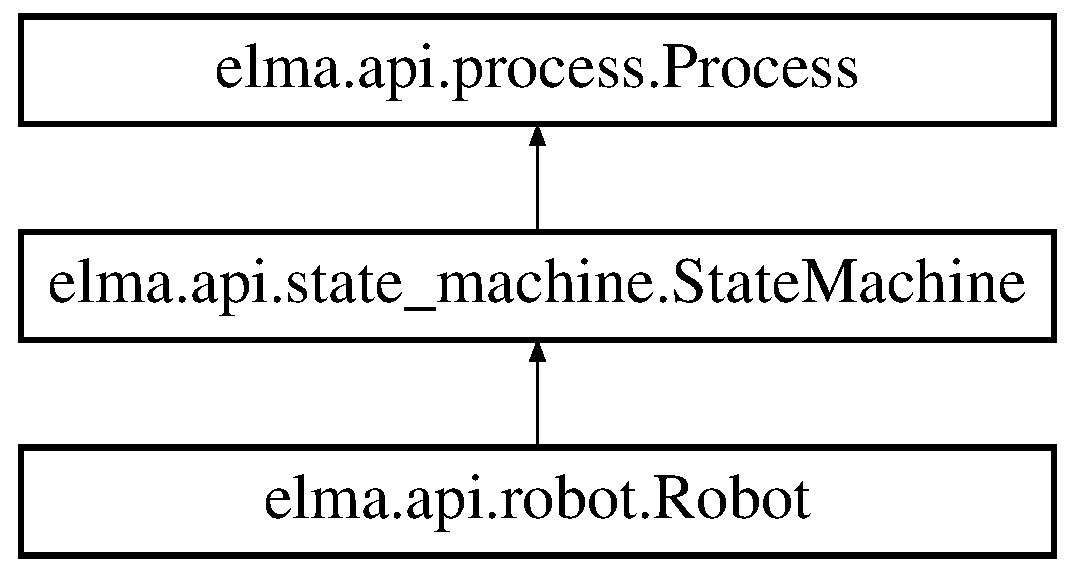
\includegraphics[height=3.000000cm]{classelma_1_1api_1_1robot_1_1Robot}
\end{center}
\end{figure}
\subsection*{Public Member Functions}
\begin{DoxyCompactItemize}
\item 
\mbox{\Hypertarget{classelma_1_1api_1_1robot_1_1Robot_aa569723562580d98b16ef858b85c5154}\label{classelma_1_1api_1_1robot_1_1Robot_aa569723562580d98b16ef858b85c5154}} 
def {\bfseries \+\_\+\+\_\+init\+\_\+\+\_\+} (self, name=\char`\"{}\char`\"{})
\end{DoxyCompactItemize}
\subsection*{Public Attributes}
\begin{DoxyCompactItemize}
\item 
\mbox{\Hypertarget{classelma_1_1api_1_1robot_1_1Robot_ab1fa357b053ae9c5a0619689698e9bbc}\label{classelma_1_1api_1_1robot_1_1Robot_ab1fa357b053ae9c5a0619689698e9bbc}} 
{\bfseries recharge}
\item 
\mbox{\Hypertarget{classelma_1_1api_1_1robot_1_1Robot_ad527326117d39ba9cad2d3673df59ca6}\label{classelma_1_1api_1_1robot_1_1Robot_ad527326117d39ba9cad2d3673df59ca6}} 
{\bfseries wander}
\item 
\mbox{\Hypertarget{classelma_1_1api_1_1robot_1_1Robot_a6b9bc3b5714ccfadf434c266e6f42639}\label{classelma_1_1api_1_1robot_1_1Robot_a6b9bc3b5714ccfadf434c266e6f42639}} 
{\bfseries find\+\_\+recharge\+\_\+station}
\item 
\mbox{\Hypertarget{classelma_1_1api_1_1robot_1_1Robot_a31f1c867344f45e87b6dfe9d958d13dd}\label{classelma_1_1api_1_1robot_1_1Robot_a31f1c867344f45e87b6dfe9d958d13dd}} 
{\bfseries evade}
\item 
\mbox{\Hypertarget{classelma_1_1api_1_1robot_1_1Robot_a7314c2483ca6d96cf75016cb4e7cf43e}\label{classelma_1_1api_1_1robot_1_1Robot_a7314c2483ca6d96cf75016cb4e7cf43e}} 
{\bfseries make\+\_\+noise}
\end{DoxyCompactItemize}


The documentation for this class was generated from the following file\+:\begin{DoxyCompactItemize}
\item 
elma/api/robot.\+py\end{DoxyCompactItemize}

\hypertarget{classelma_1_1api_1_1robot_1_1RobotState}{}\section{elma.\+api.\+robot.\+Robot\+State Class Reference}
\label{classelma_1_1api_1_1robot_1_1RobotState}\index{elma.\+api.\+robot.\+Robot\+State@{elma.\+api.\+robot.\+Robot\+State}}
Inheritance diagram for elma.\+api.\+robot.\+Robot\+State\+:\begin{figure}[H]
\begin{center}
\leavevmode
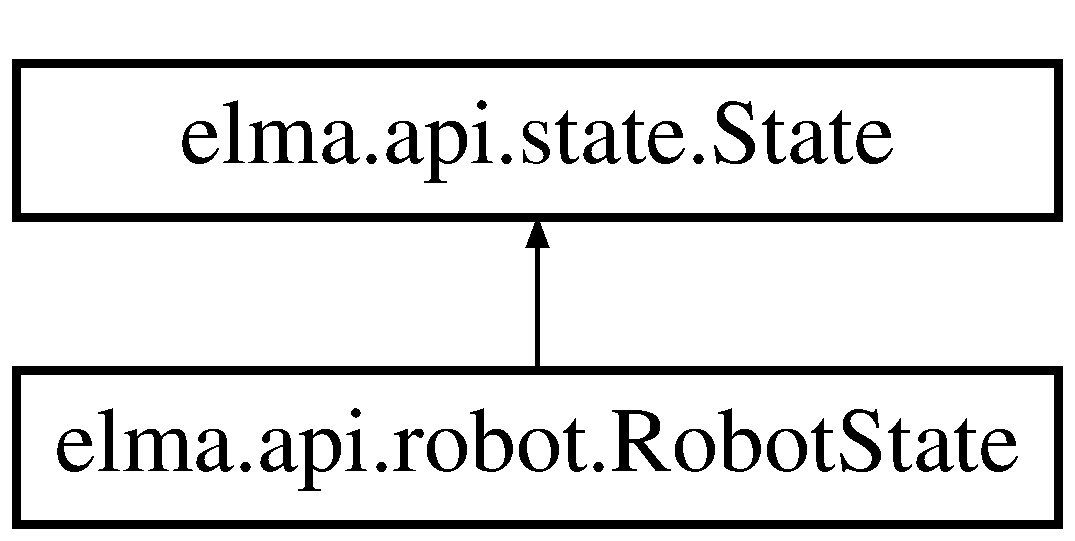
\includegraphics[height=2.000000cm]{classelma_1_1api_1_1robot_1_1RobotState}
\end{center}
\end{figure}
\subsection*{Public Member Functions}
\begin{DoxyCompactItemize}
\item 
\mbox{\Hypertarget{classelma_1_1api_1_1robot_1_1RobotState_a1499921c2c3d6b51569be5cfbcad1085}\label{classelma_1_1api_1_1robot_1_1RobotState_a1499921c2c3d6b51569be5cfbcad1085}} 
def {\bfseries \+\_\+\+\_\+init\+\_\+\+\_\+} (self, name)
\item 
\mbox{\Hypertarget{classelma_1_1api_1_1robot_1_1RobotState_a13a44c6ec8836f2235982916b615c977}\label{classelma_1_1api_1_1robot_1_1RobotState_a13a44c6ec8836f2235982916b615c977}} 
def {\bfseries entry} (self, event)
\item 
\mbox{\Hypertarget{classelma_1_1api_1_1robot_1_1RobotState_afc16183bb851de813f3269937c2360a6}\label{classelma_1_1api_1_1robot_1_1RobotState_afc16183bb851de813f3269937c2360a6}} 
def {\bfseries during} (self)
\item 
\mbox{\Hypertarget{classelma_1_1api_1_1robot_1_1RobotState_aa9054b608060dd161e4a18f194f62689}\label{classelma_1_1api_1_1robot_1_1RobotState_aa9054b608060dd161e4a18f194f62689}} 
def {\bfseries exit} (self, event)
\end{DoxyCompactItemize}


The documentation for this class was generated from the following file\+:\begin{DoxyCompactItemize}
\item 
elma/api/robot.\+py\end{DoxyCompactItemize}

\hypertarget{classelma_1_1api_1_1state_1_1State}{}\section{elma.\+api.\+state.\+State Class Reference}
\label{classelma_1_1api_1_1state_1_1State}\index{elma.\+api.\+state.\+State@{elma.\+api.\+state.\+State}}


A class which represents a \hyperlink{classelma_1_1api_1_1state_1_1State}{State} in the Finite \hyperlink{classelma_1_1api_1_1state_1_1State}{State} Machine.  


Inheritance diagram for elma.\+api.\+state.\+State\+:\begin{figure}[H]
\begin{center}
\leavevmode
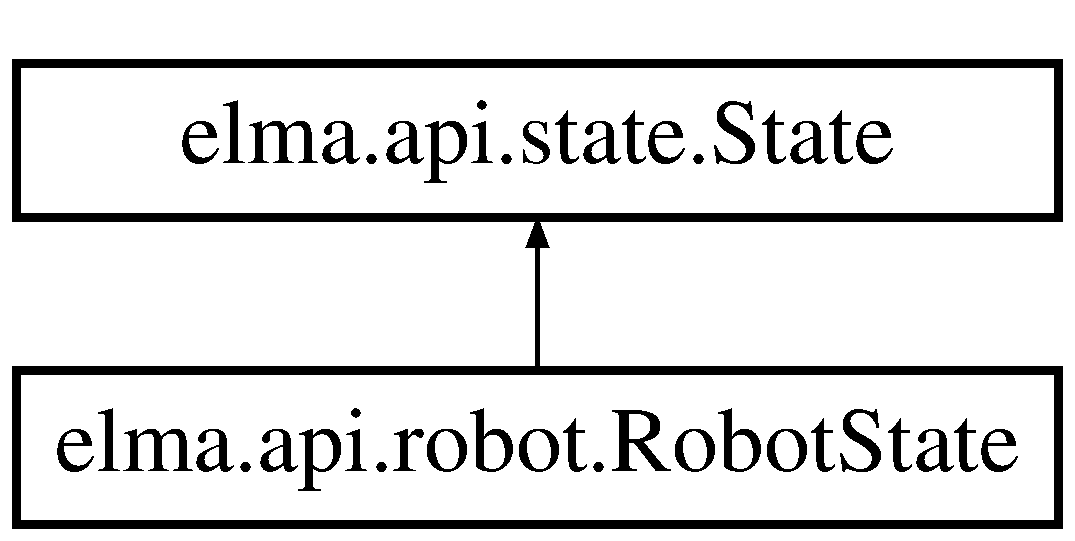
\includegraphics[height=2.000000cm]{classelma_1_1api_1_1state_1_1State}
\end{center}
\end{figure}
\subsection*{Public Member Functions}
\begin{DoxyCompactItemize}
\item 
\mbox{\Hypertarget{classelma_1_1api_1_1state_1_1State_a527faccc6a4e00fff27b66ac685a2dbb}\label{classelma_1_1api_1_1state_1_1State_a527faccc6a4e00fff27b66ac685a2dbb}} 
def {\bfseries \+\_\+\+\_\+init\+\_\+\+\_\+} (self, \hyperlink{classelma_1_1api_1_1state_1_1State_af557d974acb64b3cd0b6bc687bb1658a}{name}=\char`\"{}unnamed state\char`\"{})
\item 
def \hyperlink{classelma_1_1api_1_1state_1_1State_af557d974acb64b3cd0b6bc687bb1658a}{name} (self)
\item 
def \hyperlink{classelma_1_1api_1_1state_1_1State_aad456a6f35fb49f1e1702eac0954ed2c}{id} (self)
\item 
def \hyperlink{classelma_1_1api_1_1state_1_1State_a9faa0f15ba6f380e9815554cdbfd586d}{entry} (self, event)
\begin{DoxyCompactList}\small\item\em A method that derived instances should define. \end{DoxyCompactList}\item 
def \hyperlink{classelma_1_1api_1_1state_1_1State_a67235fad4e69aa8c21ec26eae249e01d}{during} (self, event)
\begin{DoxyCompactList}\small\item\em A method that derived instances should define. \end{DoxyCompactList}\item 
def \hyperlink{classelma_1_1api_1_1state_1_1State_ad57604af6fe62f311bc073cf027ea552}{exit} (self, event)
\begin{DoxyCompactList}\small\item\em A method that derived instances should define. \end{DoxyCompactList}\end{DoxyCompactItemize}


\subsection{Detailed Description}
A class which represents a \hyperlink{classelma_1_1api_1_1state_1_1State}{State} in the Finite \hyperlink{classelma_1_1api_1_1state_1_1State}{State} Machine. 



\subsection{Member Function Documentation}
\mbox{\Hypertarget{classelma_1_1api_1_1state_1_1State_a67235fad4e69aa8c21ec26eae249e01d}\label{classelma_1_1api_1_1state_1_1State_a67235fad4e69aa8c21ec26eae249e01d}} 
\index{elma\+::api\+::state\+::\+State@{elma\+::api\+::state\+::\+State}!during@{during}}
\index{during@{during}!elma\+::api\+::state\+::\+State@{elma\+::api\+::state\+::\+State}}
\subsubsection{\texorpdfstring{during()}{during()}}
{\footnotesize\ttfamily def elma.\+api.\+state.\+State.\+during (\begin{DoxyParamCaption}\item[{}]{self,  }\item[{}]{event }\end{DoxyParamCaption})}



A method that derived instances should define. 

It is called repeatedly by the update() method of the containing State\+Machine when the state is active. \mbox{\Hypertarget{classelma_1_1api_1_1state_1_1State_a9faa0f15ba6f380e9815554cdbfd586d}\label{classelma_1_1api_1_1state_1_1State_a9faa0f15ba6f380e9815554cdbfd586d}} 
\index{elma\+::api\+::state\+::\+State@{elma\+::api\+::state\+::\+State}!entry@{entry}}
\index{entry@{entry}!elma\+::api\+::state\+::\+State@{elma\+::api\+::state\+::\+State}}
\subsubsection{\texorpdfstring{entry()}{entry()}}
{\footnotesize\ttfamily def elma.\+api.\+state.\+State.\+entry (\begin{DoxyParamCaption}\item[{}]{self,  }\item[{}]{event }\end{DoxyParamCaption})}



A method that derived instances should define. 

It is called when the state is entered by the state machine either when the machine starts or when a transition to the state is fired. 
\begin{DoxyParams}{Parameters}
{\em e} & The event that led to the transition into the state \\
\hline
\end{DoxyParams}
\mbox{\Hypertarget{classelma_1_1api_1_1state_1_1State_ad57604af6fe62f311bc073cf027ea552}\label{classelma_1_1api_1_1state_1_1State_ad57604af6fe62f311bc073cf027ea552}} 
\index{elma\+::api\+::state\+::\+State@{elma\+::api\+::state\+::\+State}!exit@{exit}}
\index{exit@{exit}!elma\+::api\+::state\+::\+State@{elma\+::api\+::state\+::\+State}}
\subsubsection{\texorpdfstring{exit()}{exit()}}
{\footnotesize\ttfamily def elma.\+api.\+state.\+State.\+exit (\begin{DoxyParamCaption}\item[{}]{self,  }\item[{}]{event }\end{DoxyParamCaption})}



A method that derived instances should define. 

It is called just before the state is exited by the state machine when a transition from the state is fired. 
\begin{DoxyParams}{Parameters}
{\em e} & The event that led to the transition out of the state \\
\hline
\end{DoxyParams}
\mbox{\Hypertarget{classelma_1_1api_1_1state_1_1State_aad456a6f35fb49f1e1702eac0954ed2c}\label{classelma_1_1api_1_1state_1_1State_aad456a6f35fb49f1e1702eac0954ed2c}} 
\index{elma\+::api\+::state\+::\+State@{elma\+::api\+::state\+::\+State}!id@{id}}
\index{id@{id}!elma\+::api\+::state\+::\+State@{elma\+::api\+::state\+::\+State}}
\subsubsection{\texorpdfstring{id()}{id()}}
{\footnotesize\ttfamily def elma.\+api.\+state.\+State.\+id (\begin{DoxyParamCaption}\item[{}]{self }\end{DoxyParamCaption})}

\begin{DoxyReturn}{Returns}
The id of the state 
\end{DoxyReturn}
\mbox{\Hypertarget{classelma_1_1api_1_1state_1_1State_af557d974acb64b3cd0b6bc687bb1658a}\label{classelma_1_1api_1_1state_1_1State_af557d974acb64b3cd0b6bc687bb1658a}} 
\index{elma\+::api\+::state\+::\+State@{elma\+::api\+::state\+::\+State}!name@{name}}
\index{name@{name}!elma\+::api\+::state\+::\+State@{elma\+::api\+::state\+::\+State}}
\subsubsection{\texorpdfstring{name()}{name()}}
{\footnotesize\ttfamily def elma.\+api.\+state.\+State.\+name (\begin{DoxyParamCaption}\item[{}]{self }\end{DoxyParamCaption})}

\begin{DoxyReturn}{Returns}
The name of the state 
\end{DoxyReturn}


The documentation for this class was generated from the following file\+:\begin{DoxyCompactItemize}
\item 
elma/api/state.\+py\end{DoxyCompactItemize}

\hypertarget{classelma_1_1api_1_1state__machine_1_1StateMachine}{}\section{elma.\+api.\+state\+\_\+machine.\+State\+Machine Class Reference}
\label{classelma_1_1api_1_1state__machine_1_1StateMachine}\index{elma.\+api.\+state\+\_\+machine.\+State\+Machine@{elma.\+api.\+state\+\_\+machine.\+State\+Machine}}
Inheritance diagram for elma.\+api.\+state\+\_\+machine.\+State\+Machine\+:\begin{figure}[H]
\begin{center}
\leavevmode
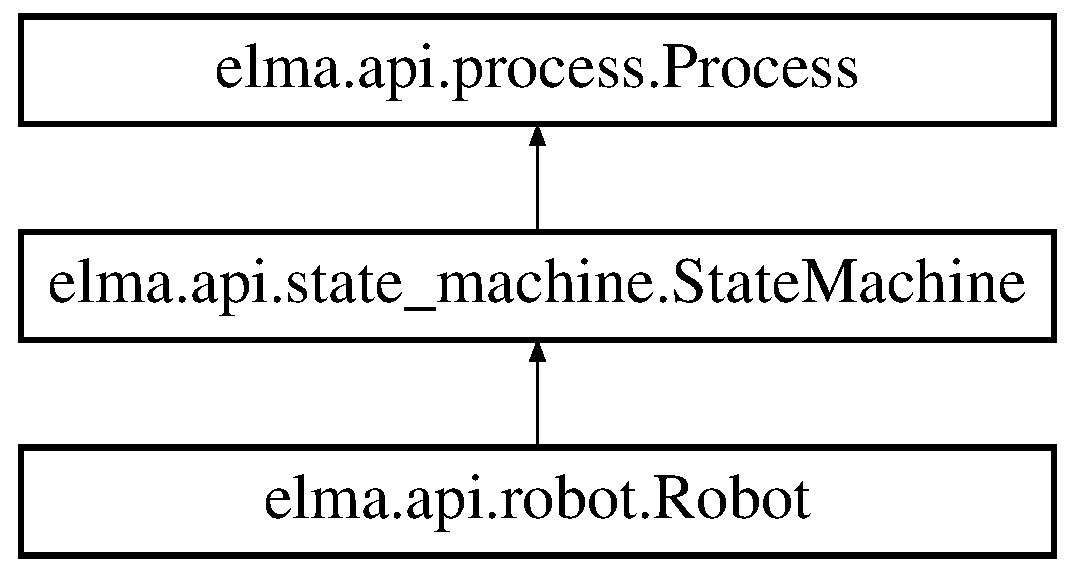
\includegraphics[height=3.000000cm]{classelma_1_1api_1_1state__machine_1_1StateMachine}
\end{center}
\end{figure}
\subsection*{Public Member Functions}
\begin{DoxyCompactItemize}
\item 
\mbox{\Hypertarget{classelma_1_1api_1_1state__machine_1_1StateMachine_ac78c9f7d441428da577f56575950df32}\label{classelma_1_1api_1_1state__machine_1_1StateMachine_ac78c9f7d441428da577f56575950df32}} 
def {\bfseries \+\_\+\+\_\+init\+\_\+\+\_\+} (self, name=\char`\"{}unnamed state machine\char`\"{})
\item 
\mbox{\Hypertarget{classelma_1_1api_1_1state__machine_1_1StateMachine_a811156049fbd4acfd8104b2d83506d3a}\label{classelma_1_1api_1_1state__machine_1_1StateMachine_a811156049fbd4acfd8104b2d83506d3a}} 
def {\bfseries set\+\_\+initial} (self, s)
\item 
\mbox{\Hypertarget{classelma_1_1api_1_1state__machine_1_1StateMachine_adfb788d612f7453935d09bc39d87aa3d}\label{classelma_1_1api_1_1state__machine_1_1StateMachine_adfb788d612f7453935d09bc39d87aa3d}} 
def {\bfseries add\+\_\+transition} (self, event\+\_\+name, from\+\_\+state, to\+\_\+state)
\item 
\mbox{\Hypertarget{classelma_1_1api_1_1state__machine_1_1StateMachine_afe81dcfc4462c855a95d0088da346f77}\label{classelma_1_1api_1_1state__machine_1_1StateMachine_afe81dcfc4462c855a95d0088da346f77}} 
def {\bfseries init} (self)
\item 
\mbox{\Hypertarget{classelma_1_1api_1_1state__machine_1_1StateMachine_aa41df28621b1c1bff35a22f4e546468d}\label{classelma_1_1api_1_1state__machine_1_1StateMachine_aa41df28621b1c1bff35a22f4e546468d}} 
def {\bfseries start} (self)
\item 
\mbox{\Hypertarget{classelma_1_1api_1_1state__machine_1_1StateMachine_ae06fd2e258a724100a32c1a2a515a415}\label{classelma_1_1api_1_1state__machine_1_1StateMachine_ae06fd2e258a724100a32c1a2a515a415}} 
def {\bfseries stop} (self)
\item 
\mbox{\Hypertarget{classelma_1_1api_1_1state__machine_1_1StateMachine_a09377453c82f6a20fa74e5b6196bbcf7}\label{classelma_1_1api_1_1state__machine_1_1StateMachine_a09377453c82f6a20fa74e5b6196bbcf7}} 
def {\bfseries update} (self)
\item 
\mbox{\Hypertarget{classelma_1_1api_1_1state__machine_1_1StateMachine_a33e5740993b92f934277ba3301854e1e}\label{classelma_1_1api_1_1state__machine_1_1StateMachine_a33e5740993b92f934277ba3301854e1e}} 
def {\bfseries set\+\_\+propagate} (self, val)
\item 
\mbox{\Hypertarget{classelma_1_1api_1_1state__machine_1_1StateMachine_a2901d43df138803f6763c96823369242}\label{classelma_1_1api_1_1state__machine_1_1StateMachine_a2901d43df138803f6763c96823369242}} 
def {\bfseries current} (self)
\end{DoxyCompactItemize}
\subsection*{Additional Inherited Members}


The documentation for this class was generated from the following file\+:\begin{DoxyCompactItemize}
\item 
elma/api/state\+\_\+machine.\+py\end{DoxyCompactItemize}

\hypertarget{classelma_1_1api_1_1process_1_1Status__Type}{}\section{elma.\+api.\+process.\+Status\+\_\+\+Type Class Reference}
\label{classelma_1_1api_1_1process_1_1Status__Type}\index{elma.\+api.\+process.\+Status\+\_\+\+Type@{elma.\+api.\+process.\+Status\+\_\+\+Type}}
Inheritance diagram for elma.\+api.\+process.\+Status\+\_\+\+Type\+:\begin{figure}[H]
\begin{center}
\leavevmode
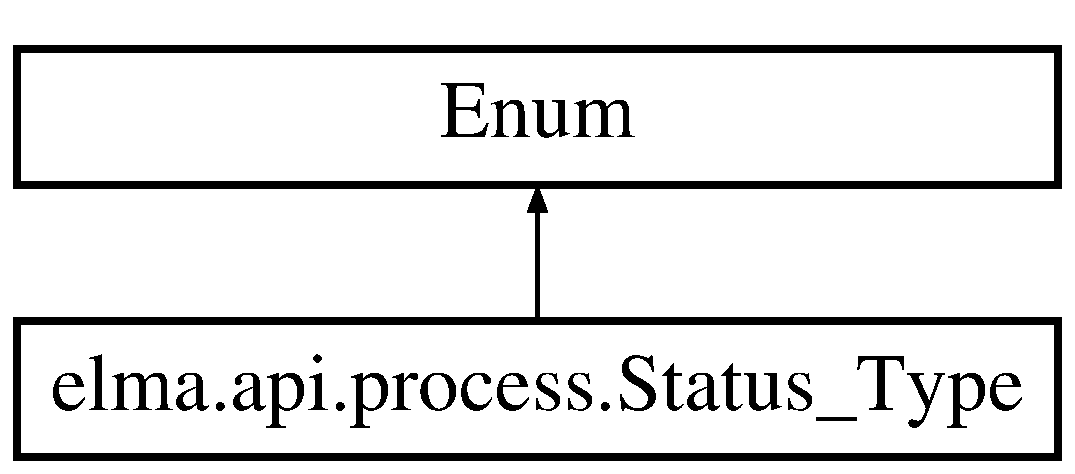
\includegraphics[height=2.000000cm]{classelma_1_1api_1_1process_1_1Status__Type}
\end{center}
\end{figure}
\subsection*{Static Public Attributes}
\begin{DoxyCompactItemize}
\item 
\mbox{\Hypertarget{classelma_1_1api_1_1process_1_1Status__Type_a3931e54de54d07963d9f7a2896964231}\label{classelma_1_1api_1_1process_1_1Status__Type_a3931e54de54d07963d9f7a2896964231}} 
int {\bfseries U\+N\+I\+N\+I\+T\+I\+A\+L\+I\+Z\+ED} = 1
\item 
\mbox{\Hypertarget{classelma_1_1api_1_1process_1_1Status__Type_a3069b069e3cd2d3a36a471a1d84d1738}\label{classelma_1_1api_1_1process_1_1Status__Type_a3069b069e3cd2d3a36a471a1d84d1738}} 
int {\bfseries S\+T\+O\+P\+P\+ED} = 2
\item 
\mbox{\Hypertarget{classelma_1_1api_1_1process_1_1Status__Type_acad68ee8aaa785f6adabec51c3c19207}\label{classelma_1_1api_1_1process_1_1Status__Type_acad68ee8aaa785f6adabec51c3c19207}} 
int {\bfseries R\+U\+N\+N\+I\+NG} = 3
\end{DoxyCompactItemize}


The documentation for this class was generated from the following file\+:\begin{DoxyCompactItemize}
\item 
elma/api/process.\+py\end{DoxyCompactItemize}

\hypertarget{classelma_1_1test_1_1test__elma_1_1TestElma}{}\section{elma.\+test.\+test\+\_\+elma.\+Test\+Elma Class Reference}
\label{classelma_1_1test_1_1test__elma_1_1TestElma}\index{elma.\+test.\+test\+\_\+elma.\+Test\+Elma@{elma.\+test.\+test\+\_\+elma.\+Test\+Elma}}
Inheritance diagram for elma.\+test.\+test\+\_\+elma.\+Test\+Elma\+:\begin{figure}[H]
\begin{center}
\leavevmode
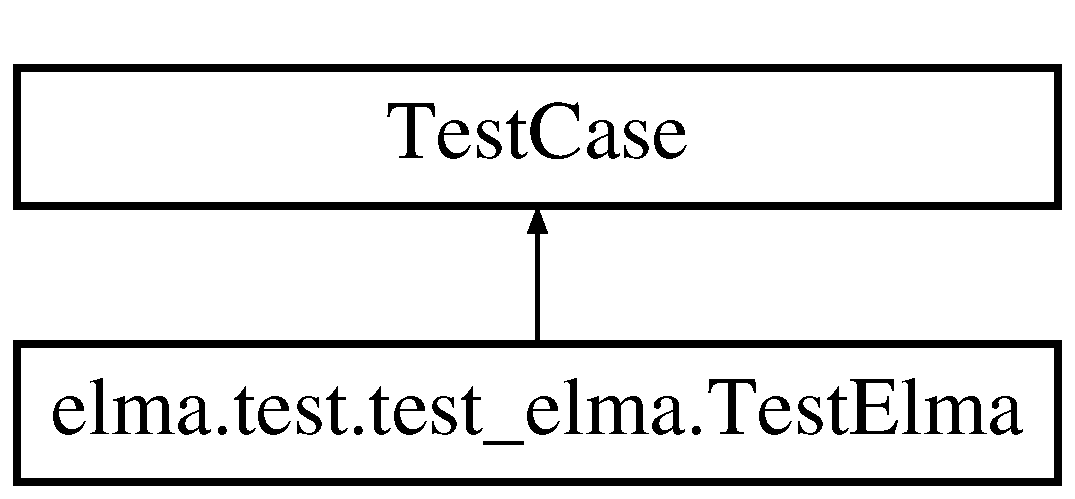
\includegraphics[height=2.000000cm]{classelma_1_1test_1_1test__elma_1_1TestElma}
\end{center}
\end{figure}
\subsection*{Public Member Functions}
\begin{DoxyCompactItemize}
\item 
\mbox{\Hypertarget{classelma_1_1test_1_1test__elma_1_1TestElma_a08a7479359af5f71989bd49ed065391b}\label{classelma_1_1test_1_1test__elma_1_1TestElma_a08a7479359af5f71989bd49ed065391b}} 
def {\bfseries test\+\_\+process} (self)
\item 
\mbox{\Hypertarget{classelma_1_1test_1_1test__elma_1_1TestElma_a168e8341dac5e84682a83c7dd93c5cc7}\label{classelma_1_1test_1_1test__elma_1_1TestElma_a168e8341dac5e84682a83c7dd93c5cc7}} 
def {\bfseries test\+\_\+robot} (self)
\item 
\mbox{\Hypertarget{classelma_1_1test_1_1test__elma_1_1TestElma_a295c71bd47bb411f73b9715f5846ae2c}\label{classelma_1_1test_1_1test__elma_1_1TestElma_a295c71bd47bb411f73b9715f5846ae2c}} 
def {\bfseries test\+\_\+robot\+\_\+two} (self)
\end{DoxyCompactItemize}


The documentation for this class was generated from the following file\+:\begin{DoxyCompactItemize}
\item 
elma/test/test\+\_\+elma.\+py\end{DoxyCompactItemize}

\hypertarget{classelma_1_1test_1_1test__process_1_1TestProcess}{}\section{elma.\+test.\+test\+\_\+process.\+Test\+Process Class Reference}
\label{classelma_1_1test_1_1test__process_1_1TestProcess}\index{elma.\+test.\+test\+\_\+process.\+Test\+Process@{elma.\+test.\+test\+\_\+process.\+Test\+Process}}


This is a test process class inheriting the Process class to test the working of the E\+L\+MA process A\+P\+Is.  


Inheritance diagram for elma.\+test.\+test\+\_\+process.\+Test\+Process\+:\begin{figure}[H]
\begin{center}
\leavevmode
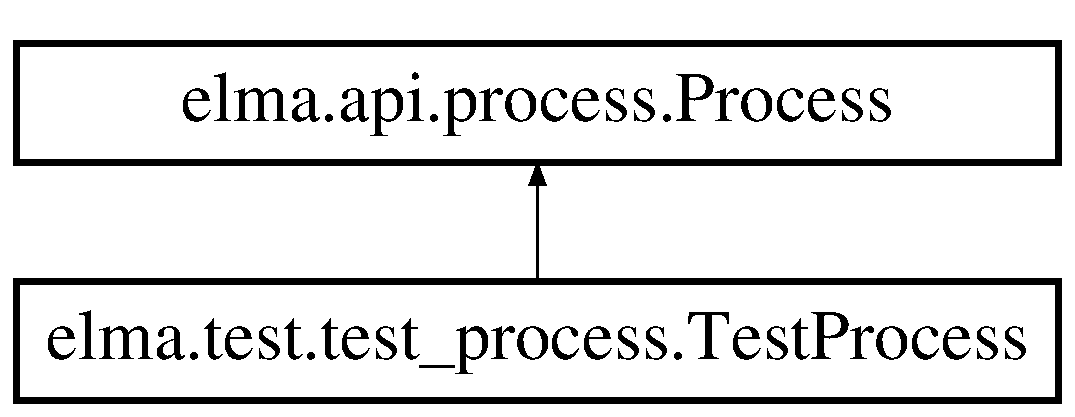
\includegraphics[height=2.000000cm]{classelma_1_1test_1_1test__process_1_1TestProcess}
\end{center}
\end{figure}
\subsection*{Public Member Functions}
\begin{DoxyCompactItemize}
\item 
\mbox{\Hypertarget{classelma_1_1test_1_1test__process_1_1TestProcess_a84bfdbfccb64a0936b5ebefe85adf1a9}\label{classelma_1_1test_1_1test__process_1_1TestProcess_a84bfdbfccb64a0936b5ebefe85adf1a9}} 
def {\bfseries \+\_\+\+\_\+init\+\_\+\+\_\+} (self, \hyperlink{classelma_1_1api_1_1process_1_1Process_affa061fab12e699d4d04471bfaf52a1a}{name}=None, \hyperlink{classelma_1_1api_1_1process_1_1Process_a6dc2725cd3d032b3ec80e0fc6c52a994}{status}=None, manager=None)
\item 
\mbox{\Hypertarget{classelma_1_1test_1_1test__process_1_1TestProcess_af89f2474553f0246a4a71aa5abc6c038}\label{classelma_1_1test_1_1test__process_1_1TestProcess_af89f2474553f0246a4a71aa5abc6c038}} 
def {\bfseries hello} (self, e)
\item 
\mbox{\Hypertarget{classelma_1_1test_1_1test__process_1_1TestProcess_afc1162f9234c83f55a942fc50acc921e}\label{classelma_1_1test_1_1test__process_1_1TestProcess_afc1162f9234c83f55a942fc50acc921e}} 
def {\bfseries pi} (self, e)
\item 
\mbox{\Hypertarget{classelma_1_1test_1_1test__process_1_1TestProcess_a26a44df47fb0758cf808c9efe4c39bfc}\label{classelma_1_1test_1_1test__process_1_1TestProcess_a26a44df47fb0758cf808c9efe4c39bfc}} 
def {\bfseries init} (self)
\item 
\mbox{\Hypertarget{classelma_1_1test_1_1test__process_1_1TestProcess_a4475739a2b7898dd5d138cc7c59879d9}\label{classelma_1_1test_1_1test__process_1_1TestProcess_a4475739a2b7898dd5d138cc7c59879d9}} 
def {\bfseries start} (self)
\item 
\mbox{\Hypertarget{classelma_1_1test_1_1test__process_1_1TestProcess_a55c1cee8682fe48db1649fd1f1aa603f}\label{classelma_1_1test_1_1test__process_1_1TestProcess_a55c1cee8682fe48db1649fd1f1aa603f}} 
def {\bfseries update} (self)
\item 
\mbox{\Hypertarget{classelma_1_1test_1_1test__process_1_1TestProcess_a2c4a784c3c7531220cf114f6bf84b5af}\label{classelma_1_1test_1_1test__process_1_1TestProcess_a2c4a784c3c7531220cf114f6bf84b5af}} 
def {\bfseries stop} (self)
\end{DoxyCompactItemize}
\subsection*{Public Attributes}
\begin{DoxyCompactItemize}
\item 
\mbox{\Hypertarget{classelma_1_1test_1_1test__process_1_1TestProcess_a206dcaf5ce8086f6ddc812c5d5c06ff7}\label{classelma_1_1test_1_1test__process_1_1TestProcess_a206dcaf5ce8086f6ddc812c5d5c06ff7}} 
{\bfseries str}
\item 
\mbox{\Hypertarget{classelma_1_1test_1_1test__process_1_1TestProcess_a2c109ab29963b2037822f52a3ec93784}\label{classelma_1_1test_1_1test__process_1_1TestProcess_a2c109ab29963b2037822f52a3ec93784}} 
{\bfseries x}
\end{DoxyCompactItemize}


\subsection{Detailed Description}
This is a test process class inheriting the Process class to test the working of the E\+L\+MA process A\+P\+Is. 



The documentation for this class was generated from the following file\+:\begin{DoxyCompactItemize}
\item 
elma/test/test\+\_\+process.\+py\end{DoxyCompactItemize}

\hypertarget{classelma_1_1api_1_1transition_1_1Transition}{}\section{elma.\+api.\+transition.\+Transition Class Reference}
\label{classelma_1_1api_1_1transition_1_1Transition}\index{elma.\+api.\+transition.\+Transition@{elma.\+api.\+transition.\+Transition}}
\subsection*{Public Member Functions}
\begin{DoxyCompactItemize}
\item 
\mbox{\Hypertarget{classelma_1_1api_1_1transition_1_1Transition_a7356a55e17ab1c10419e4b61a778e08e}\label{classelma_1_1api_1_1transition_1_1Transition_a7356a55e17ab1c10419e4b61a778e08e}} 
def {\bfseries \+\_\+\+\_\+init\+\_\+\+\_\+} (self, event\+\_\+name, from\+\_\+state, to\+\_\+state)
\item 
\mbox{\Hypertarget{classelma_1_1api_1_1transition_1_1Transition_a123ea144d7e16b79186865203cbc3dd4}\label{classelma_1_1api_1_1transition_1_1Transition_a123ea144d7e16b79186865203cbc3dd4}} 
def {\bfseries from\+\_\+state} (self)
\item 
\mbox{\Hypertarget{classelma_1_1api_1_1transition_1_1Transition_a62296c6ca7b1e1e75a1fa022be2998f6}\label{classelma_1_1api_1_1transition_1_1Transition_a62296c6ca7b1e1e75a1fa022be2998f6}} 
def {\bfseries to\+\_\+state} (self)
\item 
\mbox{\Hypertarget{classelma_1_1api_1_1transition_1_1Transition_a198b5050c2e6943c365fdc611aa81841}\label{classelma_1_1api_1_1transition_1_1Transition_a198b5050c2e6943c365fdc611aa81841}} 
def {\bfseries event\+\_\+name} (self)
\end{DoxyCompactItemize}


The documentation for this class was generated from the following file\+:\begin{DoxyCompactItemize}
\item 
elma/api/transition.\+py\end{DoxyCompactItemize}

%--- End generated contents ---

% Index
\backmatter
\newpage
\phantomsection
\clearemptydoublepage
\addcontentsline{toc}{chapter}{Index}
\printindex

\end{document}
